% NOTE (15 Sept 2026): archived IEEEtran version. The title is kept in
% sync, but the body predates the advisor's 15 Sept revision (unigram
% frequency-prior terminology, softened single-seed wording, Table II
% Delta_B/Delta_P columns, corrected morphology probability and early
% stopping description). paper.tex (IJPRAI) is the maintained version.
%%%%%%%%%%%%%%%%%%%%%%%%%%%%%%%%%%%%%%%%%%%%%%%%%%%%%%%%%%%%%%%%%%%%%%%%%%%%%%%
% Coverage Decides the Sign, Frequency the Size: Decomposing
%            Lexicon-Assisted Correction for Handwritten Word Recognition
%            on IAM (Aachen writer-disjoint)
% Authors: Nur Banu Oğur (corresponding), Rıdvan Dursun, Berhat Yeşilyurt
%          Dept. of Software Engineering, Sakarya University
% Template: IEEE Conference (IEEEtran)
%
% MODEL NAMING (used consistently throughout the paper):
%   no augmentation           = zero-augmentation anchor (positive control)
%   CRNN-B                    = baseline optical model, conventional augmentation
%   + wide photometric / + elastic / + morphological = ablation variants
%   CRNN-G                    = all augmentations, lexicon-free (greedy CTC)
%   CRNN-LX (PROPOSED)        = CRNN-G + lexicon-extended n-gram post-correction
%
% ALL NUMBERS: full IAM labels, Aachen writer-disjoint split, N_test = 20,310,
% six configurations trained from scratch on one machine with one code
% revision. Sources: results/ABLATION_SONUC.md, results/ablation_lexicon_*.json
%%%%%%%%%%%%%%%%%%%%%%%%%%%%%%%%%%%%%%%%%%%%%%%%%%%%%%%%%%%%%%%%%%%%%%%%%%%%%%%

\documentclass[conference]{IEEEtran}
\IEEEoverridecommandlockouts

% ---- Packages ------------------------------------------------------------
\usepackage[utf8]{inputenc}
\usepackage[T1]{fontenc}
\usepackage{cite}
\usepackage{amsmath,amssymb,amsfonts}
\usepackage{graphicx}
\usepackage{textcomp}
\usepackage{xcolor}
\usepackage{booktabs}
\usepackage{url}
\usepackage{hyperref}
\hypersetup{colorlinks=true, urlcolor=blue, citecolor=blue, linkcolor=black}

% ---- Custom commands ------------------------------------------------------
\newcommand{\ours}{CRNN-LX}            % proposed system (lexicon-extended)
\newcommand{\oursnolm}{CRNN-G}         % same optical model, greedy, no lexicon
\newcommand{\ourwa}{80.74\%}
\newcommand{\ourci}{[80.19\%, 81.28\%]}
\newcommand{\ourcer}{9.09\%}
\newcommand{\rawwa}{78.83\%}
\newcommand{\rawcer}{8.60\%}
\newcommand{\baselinewa}{80.36\%}
\newcommand{\deltawa}{0.38\,pp}
\newcommand{\nsamples}{20{,}310}

\begin{document}

% ---- Title ---------------------------------------------------------------
\title{Decomposing Lexicon-Assisted Correction for Isolated\\
       Handwritten Word Recognition on IAM: Effects of\\
       Lexicon Coverage and Frequency-Based Ranking}

\author{
\IEEEauthorblockN{Nur Banu Oğur\textsuperscript{*}, Rıdvan Dursun, Berhat Yeşilyurt}
\IEEEauthorblockA{Department of Software Engineering,
                  Faculty of Computer and Information Sciences\\
                  Sakarya University, 54050 Sakarya, Türkiye\\
% DOGRULA: Berhat'in kurumsal e-postasi kurum kalibindan turetildi, teyit edilmeli.
                  nbogur@sakarya.edu.tr,
                  ridvan.dursun@ogr.sakarya.edu.tr,
                  berhat.yesilyurt@ogr.sakarya.edu.tr
\thanks{\textsuperscript{*}Corresponding author: Nur Banu Oğur
        (nbogur@sakarya.edu.tr).}}
}

\maketitle

% ---- Abstract (plain language, no formulas) ------------------------------
\begin{abstract}
Recognising isolated handwritten words is difficult mainly because
handwriting varies strongly from one writer to another. We study this
problem on the IAM database under the Aachen writer-disjoint protocol,
where no writer seen during training appears in the test set, and we
report every result on the complete test partition of \nsamples\
words. Our system, \ours, is a convolutional-recurrent network trained
from scratch and followed by a lexicon-aware post-corrector. Two
questions are examined under identical conditions. The first concerns
that post-corrector, which is usually reported as a single
``dictionary'' or ``language model'' step. Separating its two
ingredients shows that they do different jobs: the \emph{coverage} of
the lexicon decides the sign of the correction --- the 7\,K-word
training vocabulary alone \emph{lowers} accuracy by 2.4 points, a
239\,K-type general English list raises it by 0.7 --- while the
\emph{frequency prior} used to rank the candidates within edit
distance supplies most of the magnitude, a further 1.2 points, and is
worth twice as much on the large lexicon as on the small one. Together
they move accuracy from \rawwa\ to \ourwa, at the cost of a slightly
higher character error rate. The second question is whether a
``writing-aware'' augmentation scheme --- elastic stroke deformation and
morphological changes of pen thickness on top of a conventional
geometric and photometric pipeline --- improves recognition. Training
six configurations that differ only in the augmentation, we find that
it does not: every variant built on the conventional pipeline reaches
80.3--80.7\% word accuracy with no statistically significant
difference between them, whereas switching that conventional pipeline
off costs 2.5 points ($p=2\times10^{-27}$). The same measurement
therefore does detect augmentation where there is an effect; the
benefit simply saturates before the transforms we proposed. We also
show that a widely used parameterisation of elastic deformation
displaces pixels by only a few hundredths of a pixel and is therefore
inactive in practice. Code, split definitions and per-word
predictions are released.
\end{abstract}

\begin{IEEEkeywords}
handwritten text recognition, lexicon-based post-correction, language
model, IAM database, convolutional-recurrent neural network,
connectionist temporal classification, data augmentation, ablation
study, writer-independent evaluation
\end{IEEEkeywords}

% ---- 1. Introduction ----------------------------------------------------
\section{Introduction}
\label{sec:intro}

Offline \emph{handwritten text recognition} (HTR) is the task of
converting a scanned image of handwriting into machine-readable text
without access to the pen trajectory. Depending on how the input is
segmented, an HTR system may operate on full pages, on text lines, or
--- as in this work --- on isolated \emph{word} images. Word-level
recognition is the harder setting per sample, because the recogniser
cannot exploit the surrounding words of a sentence to disambiguate an
unclear glyph.

The IAM Handwriting Database~\cite{marti2002iam} is the standard
benchmark for English HTR, containing roughly 115\,000 word images from
657 writers. We adopt the partition released by RWTH Aachen
University~\cite{aachen_split} --- referred to as the \emph{Aachen
split} throughout this paper --- which guarantees that no writer
contributes to more than one of the training, validation and test
sets. This \emph{writer-disjoint} protocol is stricter than a random
split and is the realistic condition for deploying a recogniser on
handwriting it has never seen.

Modern recognisers are trained with the \emph{connectionist temporal
classification} (CTC) objective~\cite{graves2006connectionist}, which
removes the need for character-level alignment between the image and
its transcription. Two model families dominate: convolutional-recurrent
networks (CRNNs) trained with CTC~\cite{shi2017crnn, puigcerver2017,
bluche2017gated}, and attention-based sequence-to-sequence or
transformer encoders~\cite{kang2018convolve, michael2019evaluating}.
For a compact CRNN, two ingredients are commonly credited with closing
part of the gap to heavier models: data augmentation that reflects how
handwriting actually varies, and a lexical prior applied at or after
decoding. Both are widely used, but their individual contribution is
rarely measured under controlled conditions --- same data, same
architecture, same training schedule, same test set.

This paper provides such a measurement, and finds the two ingredients
unequal. We name the proposed system \ours\ (CRNN with
lexicon-extended n-gram post-correction) and its lexicon-free
counterpart \oursnolm; Table~\ref{tab:naming} defines the six
configurations compared. Our contributions are:

\begin{itemize}
  \item \textbf{An anatomy of lexicon-assisted correction.} Holding the
        optical model fixed, we vary the post-correction lexicon and the
        rescoring independently, which separates two effects that are
        usually reported as one. Coverage decides the sign: the training
        vocabulary alone \emph{hurts} ($-2.4$ to $-2.7$\,pp on the five
        augmented models), a general English list helps ($+0.3$ to
        $+0.7$\,pp). The frequency prior then supplies most of the
        magnitude ($+1.1$ to $+1.3$\,pp), and its value grows with the
        lexicon, because a larger candidate set makes the ranking
        matter more. Neither ingredient alone accounts for the
        $+1.5$ to $+1.9$\,pp that the full corrector delivers.
  \item \textbf{A controlled augmentation ablation with a positive
        control.} Six networks that differ only in the augmentation
        schedule are trained from scratch on the full Aachen training
        set and evaluated on the full test set. Elastic deformation,
        morphological perturbation and a widened photometric range
        change word accuracy by at most \deltawa, and none of those
        differences is statistically significant; removing the
        conventional pipeline underneath them costs $2.49$\,pp at
        $p=2\times10^{-27}$. The null result is therefore a saturation
        effect, not an insensitive experiment.
  \item \textbf{A methodological observation on elastic deformation.}
        The common parameterisation --- normalised Gaussian-smoothed
        noise scaled by $\alpha\in[2,5]$ --- yields displacements of
        0.03--0.06 pixels RMS and is effectively a no-op; we report the
        corrected parameterisation we used and its effect.
  \item \textbf{A verified evaluation protocol and full release.}
        Writer-, prompt- and form-level disjointness of the split are
        checked programmatically; all \nsamples\ test words are used;
        code, split lists and per-word predictions are public.
\end{itemize}

Section~\ref{sec:related} groups the related literature into three
families and positions our work within them.
Section~\ref{sec:method} describes the pipeline of
Fig.~\ref{fig:pipeline}. Section~\ref{sec:experiments} formalises the
evaluation metrics and statistical tests.
Section~\ref{sec:results} reports the results,
Section~\ref{sec:discussion} analyses them, and
Section~\ref{sec:conclusion} concludes.

% ---- 2. Related Work ----------------------------------------------------
\section{Related Work}
\label{sec:related}

We organise prior work into three families according to how each
system relates to ours: (i) \emph{recurrent CTC recognisers}, which
share our optical backbone but are almost always evaluated on text
lines; (ii) \emph{attention and transformer recognisers}, which target
the same word-level task as ours but with a different, heavier
decoding paradigm; and (iii) \emph{lexicon and language-model
decoders}, which address the same problem we address with our
post-corrector but from inside the decoding loop. For each family we
state what we adopt and where we differ.

\paragraph{Recurrent CTC recognisers.}
Graves and Schmidhuber~\cite{graves2008offline} introduced
multi-dimensional long short-term memory (LSTM) networks with CTC as
an early end-to-end offline recogniser. Puigcerver~\cite{puigcerver2017}
showed that a one-dimensional bidirectional LSTM (BiLSTM) stacked on a
convolutional neural network (CNN) feature extractor matches
multi-dimensional recurrence at a fraction of the cost, defining the
canonical CRNN baseline that our architecture follows. Bluche and
Messina~\cite{bluche2017gated} added gated convolutions, and Flor et
al.~\cite{flor2020htrflor} combined a CNN with a bidirectional gated
recurrent unit (BGRU) and a language-model pipeline. Wigington et
al.~\cite{wigington2017data} studied augmentation for CNN-LSTM
recognisers and reported gains from combined transforms on IAM lines.
We adopt the CRNN backbone unchanged; our contribution lies in
measuring, rather than assuming, the effect of the augmentation and of
the lexical prior.

\paragraph{Attention and transformer recognisers.}
Sueiras et al.~\cite{sueiras2018offline} and Kang et
al.~\cite{kang2018convolve} introduced sequence-to-sequence
recognisers with content-based attention for isolated IAM words.
Kang et al.~\cite{kang2021candidate} later integrated a language model
into the decoder itself through candidate fusion, and Kass and
Vats~\cite{kass2022attentionhtr} combined a ResNet encoder,
attention decoding and transfer learning from scene-text corpora,
reporting the strongest word-level accuracy on the Aachen split that
we are aware of. These four systems share our task, metric and split
and are listed in Section~\ref{sec:results}. Transformer
architectures such as TrOCR~\cite{li2023trocr} have since lowered
line-level error rates further, but require pre-training on hundreds
of millions of synthetic lines. Multimodal large language models have
also been benchmarked on IAM~\cite{crosilla2025llmhtr}; those systems
operate on full pages and rely on proprietary pre-training corpora, so
they are not comparable to a from-scratch word recogniser.

\paragraph{Word-level CRNN systems and lexical decoders.}
Dutta et al.~\cite{dutta2018improving} improved a CNN--recurrent
neural network (RNN) hybrid with synthetic pre-training, slant
normalisation and test-time augmentation and report a 12.61\%
unconstrained word error rate on IAM words evaluated without
punctuation or letter case, a setting not on the same footing as a
case-sensitive recogniser trained from scratch. Rajesh et
al.~\cite{rajesh2022hwrcnet} re-trained that CNN--RNN together with
their own HWRCNet, a CNN--BiLSTM operating in the JPEG discrete cosine
transform (DCT) domain, on a random 95:5 partition of IAM and obtained
77.14\% and 80.08\% strict word accuracy on uncompressed images; we
note that their headline figure of 89.05\% is \emph{word accuracy with
flexibility} of two edit operations rather than strict accuracy.
Mondal et al.~\cite{mondal2022yolo} recognise IAM words lexicon-free
by detecting individual characters with a YOLOv3 detector trained on
only 1\,200 word images and report a 29.21\% word error rate on
30\,000 randomly selected test words. On the decoder side, word beam
search (WBS)~\cite{scheidl2018wbs} injects a dictionary constraint
directly into CTC beam search. We instead apply the lexical knowledge
\emph{after} greedy decoding, which lets us swap the lexicon without
retraining or re-decoding and therefore isolate its effect.

\paragraph{Positioning.}
Of the word-level systems above, only the attention-based recognisers
of Sueiras et al.~\cite{sueiras2018offline}, Kang et
al.~\cite{kang2018convolve, kang2021candidate} and Kass and
Vats~\cite{kass2022attentionhtr} are evaluated on the Aachen
writer-disjoint partition that we use; the CRNN-family results of
Rajesh et al.~\cite{rajesh2022hwrcnet} and the detector of Mondal et
al.~\cite{mondal2022yolo} use their own random partitions of IAM.
Comparisons across protocols are indicative only; the controlled
comparisons of this paper are those between our own configurations.

% ---- 3. Method ----------------------------------------------------------
\section{Proposed System}
\label{sec:method}

Fig.~\ref{fig:pipeline} shows the complete processing chain, from the
raw IAM word crops to the reported metrics, and marks the two stages
whose effect this paper measures.

\begin{figure*}[t]
\centering
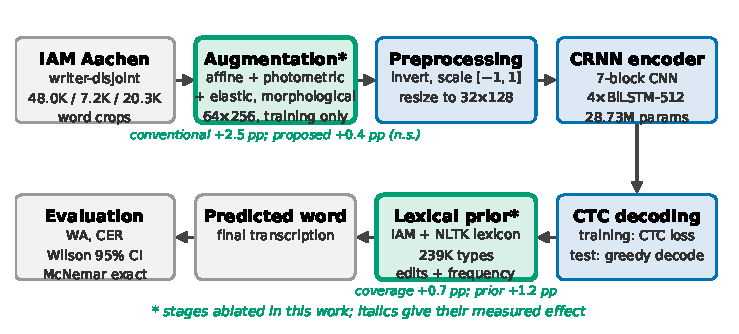
\includegraphics[width=0.92\textwidth]{figures/fig0_pipeline.pdf}
\caption{Overview of \ours. Word crops are normalised, augmented
(training only), encoded by a CRNN and decoded with CTC; the decoded
string is then corrected against a lexicon-extended n-gram language
model (LM). Green boxes mark the two stages varied in the ablations.
The evaluation stage reports word accuracy (WA), character error rate
(CER) and Wilson confidence intervals (CI), all defined formally in
Section~\ref{sec:experiments}.}
\label{fig:pipeline}
\end{figure*}

\subsection{Data and Protocol}
\label{sec:dataset}
We use the word-level IAM partition of the Aachen
split~\cite{aachen_split}: 747 training forms, 116 validation forms
and 336 test forms with disjoint writer sets (283, 55 and 161 writers
respectively). Following common practice, only word crops whose
segmentation is flagged \texttt{ok} are retained. Five validation
forms whose prompt text also occurs in the test set were removed from
the validation partition so that checkpoint selection is independent
of the test prompts; the test partition is used exactly as published.
This yields 47\,997 training words (two IAM image files are empty and
are skipped), 7\,205 validation words from 111 forms, and \nsamples\
test words from all 336 test forms. Writer, prompt and form
disjointness between the three partitions, as well as the integrity of
every record and image, are verified by a script distributed with the
code. The label alphabet contains 78 symbols (upper- and lower-case
Latin letters, digits and punctuation), plus the CTC blank.

\subsection{Model Naming}
\label{sec:naming}
Table~\ref{tab:naming} lists every configuration evaluated. All six
share the optical model of Section~\ref{sec:model}, the training
schedule and the post-corrector of Section~\ref{sec:trigram}; they
differ only in the augmentation applied during training. \oursnolm\ is
the fully augmented optical model decoded greedily, without any
lexicon; \ours\ is that same model followed by the extended-lexicon
n-gram post-corrector of Section~\ref{sec:trigram}, and is the
configuration we propose. The suffixes denote the post-processing rather than the
augmentation, which turns out not to matter (Section~\ref{sec:res-aug}). The first row is
the zero-augmentation anchor, with the conventional pipeline switched
off as well; it separates ``the proposed transforms add nothing'' from
``this pipeline detects nothing''.

\begin{table}[t]
\caption{Configurations compared. All use the same 28.73\,M-parameter
network, the same schedule and the same post-corrector.}
\label{tab:naming}
\centering
\resizebox{\columnwidth}{!}{%
\begin{tabular}{lcccc}
\toprule
Name & Conventional & Wide photometric & Elastic & Morphological \\
\midrule
no augmentation            & no  & no  & no  & no  \\
CRNN-B (baseline)          & yes & no  & no  & no  \\
$+$ wide photometric       & yes & yes & no  & no  \\
$+$ elastic                & yes & yes & yes & no  \\
$+$ morphological          & yes & yes & no  & yes \\
\textbf{\ours} (proposed)  & yes & yes & yes & yes \\
\bottomrule
\end{tabular}}
\end{table}

\subsection{Optical Model}
\label{sec:model}
The encoder is a seven-block convolutional feature extractor that
collapses the input to a single row of 512-dimensional frames,
followed by a four-layer bidirectional LSTM with 512 hidden units and
a linear projection onto the 79 output classes; the network has
28.73\,M parameters. Inputs are grayscale crops resized to
$32\times128$, inverted so that ink is high-valued, and scaled to
$[-1,1]$. The network is trained with the CTC
objective~\cite{graves2006connectionist} using AdamW with learning
rate $\eta=7\times10^{-4}$ and weight decay $10^{-5}$, five warm-up
epochs followed by cosine decay, mixed precision, and batches of 128,
for at most 100 epochs. Training stops when validation word accuracy
has not improved for 15 epochs, and the checkpoint with the best
validation word accuracy is evaluated once on the test set.

\subsection{Augmentation}
\label{sec:aug}
The baseline (CRNN-B) uses a conventional pipeline: rotation
($\pm7^\circ$), translation ($\pm5\%$), scaling ($0.9$--$1.1$), shear
($\pm5^\circ$), brightness and contrast jitter ($0.85$--$1.15$),
Gaussian noise ($\sigma=0.03$), gamma correction ($0.80$--$1.20$) and
random erasing. The ablation variants add, cumulatively:

\begin{itemize}
  \item \textbf{Wide photometric range.} Brightness and contrast
        $0.70$--$1.35$, gamma $0.70$--$1.30$, noise $\sigma=0.05$.
  \item \textbf{Elastic deformation} (probability $0.5$). A random
        displacement field is smoothed with a Gaussian kernel whose
        width is $8\%$ of the larger image side, rescaled to unit RMS,
        and multiplied by an amplitude drawn uniformly from $[1,3]$
        pixels; the crop is warped accordingly. The unit-RMS
        normalisation is essential: the frequently used variant that
        multiplies the \emph{unnormalised} blurred noise by
        $\alpha\in[2,5]$~\cite{simard2003best} produces, at this image
        size, displacements of only 0.03--0.06 pixels RMS (at most
        0.19\,px), i.e.\ it leaves the image visually and numerically
        unchanged. Our own earlier implementation had this property.
  \item \textbf{Morphological perturbation} (probability $0.3$). The
        crop is eroded or dilated with a $2\times2$ kernel,
        reproducing the difference between a fine and a broad nib.
\end{itemize}

Fig.~\ref{fig:augmentation} illustrates the transforms. All
augmentation is applied on the GPU to whole batches at a working
resolution of $64\times256$ pixels (the median IAM word height is
68\,px), with independent random parameters per sample, before the
final resize to $32\times128$; the same code path is used by all six
configurations. The zero-augmentation anchor bypasses that code path
entirely, so its crops reach the network with preprocessing only.

\begin{figure}[t]
\centering
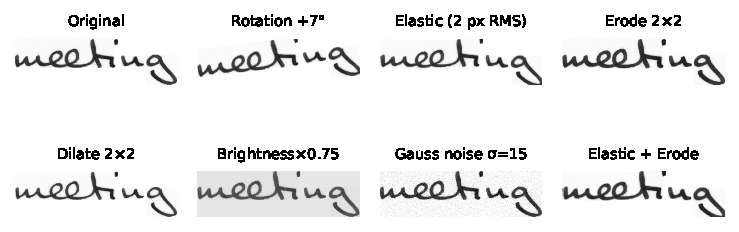
\includegraphics[width=\linewidth]{figures/fig1_augmentation_grid.pdf}
\caption{Augmentation transforms on a training crop. The elastic panel
uses the corrected amplitude (2\,px RMS); the last panel shows the
compound elastic$+$morphological effect.}
\label{fig:augmentation}
\end{figure}

\subsection{Lexicon-Extended Post-Correction}
\label{sec:trigram}
After greedy CTC decoding, each hypothesis is checked against a closed
lexicon. If the hypothesis (case-insensitively) is in the lexicon it is
accepted unchanged; otherwise it is replaced by the best-scoring
lexicon entry within a Levenshtein distance of 1 (words of up to four
characters) or 2 (longer words), where the score is the n-gram
log-probability of the candidate estimated on the IAM training
transcriptions minus a penalty of 5 per edit. The n-gram model stores
unigram, bigram and trigram counts of the 47\,997 training words (7\,173
types); because isolated word images provide no left context, the
score reduces in practice to a unigram frequency prior, and we refer to
the component as an \emph{n-gram} post-corrector.

The lexicon is the variable of interest. The \emph{training lexicon}
consists of the 7\,173 word types of the training transcriptions; the
\emph{extended lexicon} adds the Natural Language Toolkit (NLTK)
English word list, giving 239\,126 types. Measured on the test
transcriptions, the training lexicon covers 84.8\% of the test tokens
and the extended lexicon 94.0\%; the remaining tokens are proper
nouns, inflected forms absent from both lists, and punctuation-bearing
strings. Only the word \emph{list} is extended: the n-gram counts are
estimated on IAM training text alone, so no external corpus statistics
enter the model. Section~\ref{sec:results} measures the effect of each
choice with the optical model held fixed.

% ---- 4. Experimental Setup ----------------------------------------------
\section{Experimental Setup}
\label{sec:experiments}

\subsection{Evaluation Metrics}
Let $\mathcal{T}=\{(\hat{y}_i, y_i)\}_{i=1}^{N}$ be the set of
$N=\nsamples$ predicted/reference word pairs. \emph{Word accuracy}
(WA) is the exact-match rate
\begin{equation}
\mathrm{WA} \;=\; \frac{1}{N}\sum_{i=1}^{N}
      \mathbb{1}\!\left[\hat{y}_i = y_i\right],
\label{eq:wa}
\end{equation}
and the word error rate (WER) follows as
$\mathrm{WER}=1-\mathrm{WA}$. The \emph{character error rate} (CER)
aggregates Levenshtein distances $d(\cdot,\cdot)$ over the corpus,
\begin{equation}
\mathrm{CER} \;=\;
  \frac{\sum_{i=1}^{N} d(\hat{y}_i, y_i)}
       {\sum_{i=1}^{N} |y_i|},
\label{eq:cer}
\end{equation}
so that a single badly recognised long word cannot dominate the score.

\subsection{Confidence Intervals}
Because WA is a proportion estimated on a finite test set, we report
Wilson 95\% confidence intervals (CIs) rather than
normal-approximation intervals, which are unreliable near the
boundaries. For $k$ correct predictions out of $N$ and $z=1.96$,
\begin{equation}
\mathrm{CI}_{95} =
\frac{\hat{p}+\frac{z^{2}}{2N} \pm
      z\sqrt{\frac{\hat{p}(1-\hat{p})}{N}+\frac{z^{2}}{4N^{2}}}}
     {1+\frac{z^{2}}{N}},
\qquad \hat{p}=\frac{k}{N}.
\label{eq:wilson}
\end{equation}
With $N=\nsamples$ the half-width of the interval is about 0.55\,pp.

\subsection{Significance Testing}
Two systems evaluated on the same test set produce paired outcomes, so
we use the exact McNemar test. Let $b$ be the number of samples that
the first system recognises correctly and the second does not, and $c$
the converse. Under the null hypothesis the discordant pairs are
distributed $\mathrm{Bin}(b+c,\,\tfrac{1}{2})$, giving the two-sided
$p$-value
\begin{equation}
p \;=\; \min\!\left(1,\;
   2\sum_{i=0}^{\min(b,c)} \binom{b+c}{i} 2^{-(b+c)}\right).
\label{eq:mcnemar}
\end{equation}
We treat $p<0.01$ as significant.

\subsection{Reproducibility}
All six configurations were trained on the same machine (one NVIDIA
GeForce RTX~4070 Laptop GPU with 8\,GB, PyTorch~2.7.1 with CUDA~11.8,
Python~3.13) from the same code revision, with seed 42, at 35--75\,s per
epoch; a configuration takes roughly one hour. Because augmentation is
random, a single seed per configuration is used and differences
smaller than the confidence interval are not interpreted. Every number
reported below comes from one evaluation pass in single precision, in
which the six optical models and the five post-corrections are scored
against identical inputs; two independent runs of that pass agree on
all \nsamples\ hypotheses. Mixed-precision inference, by contrast, is
not bit-reproducible and shifted 2 words between runs (0.01\,pp). Code, split
definitions, the split-verification script, per-word predictions and
evaluation scripts are available at
\url{https://github.com/Ridvan013/CRNN-Handwriting-Recognition}
(branch \texttt{feature/aachen-v3-extended-trigram}); the trained
weights exceed the repository file-size limit and are distributed
separately.

% ---- 5. Results ---------------------------------------------------------
\section{Results}
\label{sec:results}

\subsection{Augmentation Ablation}
\label{sec:res-aug}

Table~\ref{tab:main} is the central result, and it separates into two
layers.

The conventional pipeline matters. Removing it costs $2.49$\,pp
(80.36 to 77.87\%) and $1.66$\,pp of character error rate; 1\,346
words are recognised only by the baseline against 840 only by the
anchor, and the exact McNemar test rejects equality at
$p=2\times10^{-27}$. Without a lexicon the same comparison is wider
still, 78.76 against 74.33\% ($-4.43$\,pp), so part of the weaker
optical model is masked by the post-corrector.

The proposed transforms do not. The five configurations that keep the
conventional pipeline reach 80.33--80.74\% and are statistically
indistinguishable: the full scheme (\ours) is nominally the best,
\deltawa\ above the baseline, but that is within one
confidence-interval half-width and no pair is rejected
($p\ge0.060$). The widened photometric range alone changes nothing
($-0.03$\,pp); elastic and morphological perturbation add $0.32$ and
$0.28$\,pp, and the two together $0.38$\,pp. On the per-word level
these five disagree on 3\,328 words (16.4\%), yet the disagreements
cancel: for the baseline--\ours\ pair, 777 words are recognised only
by the baseline and 854 only by \ours. Among configurations that
already augment, the choice of transform changes \emph{which} words are
recognised far more than \emph{how many}.

\begin{table}[t]
\caption{Augmentation ablation on the Aachen writer-disjoint test set
($N=\nsamples$). All rows share the network, schedule and
post-corrector; $p$ is the exact McNemar test against CRNN-B on
per-word outcomes. The first row is the zero-augmentation anchor and
acts as a positive control. Best validation WA and the epoch at which
it was reached are given for reference (validation: 7\,205 words, 55
writers).}
\label{tab:main}
\centering
\resizebox{\columnwidth}{!}{%
\begin{tabular}{lcccccc}
\toprule
Configuration & WA (\%) & CER (\%) & Wilson 95\% CI & $\Delta$WA & $p$ & best val WA (ep.) \\
\midrule
no augmentation        & 77.87 & 11.00 & [77.29,\,78.43] & $-2.49$ & $2\!\times\!10^{-27}$ & 82.57 (38) \\
CRNN-B (baseline)      & 80.36 & 9.34 & [79.81,\,80.90] & (ref.)  & (ref.) & 84.61 (87) \\
$+$ wide photometric   & 80.33 & 9.34 & [79.78,\,80.87] & $-0.03$ & 0.901 & 84.34 (76) \\
$+$ elastic            & 80.67 & 9.09 & [80.13,\,81.21] & $+0.32$ & 0.122 & 84.69 (77) \\
$+$ morphological      & 80.64 & 9.09 & [80.09,\,81.17] & $+0.28$ & 0.165 & 84.58 (84) \\
\textbf{\ours} (all)   & \textbf{80.74} & \textbf{9.09} & [80.19,\,81.28] & $+0.38$ & 0.060 & 84.77 (70) \\
\bottomrule
\end{tabular}}
\end{table}

Fig.~\ref{fig:curves} shows the mechanism. The anchor separates from
the rest early: it drives the training loss down to 0.018 --- a fifth
of what the augmented runs reach --- while its validation loss rises,
peaks at 82.57\% validation accuracy by epoch 38 and triggers early
stopping at epoch 53. It memorises the training set. The five
augmented runs keep improving to epoch 70--87 and converge to a
plateau of 84.3--84.8\%, and among them the curves are
indistinguishable after the first fifteen epochs; their training
losses differ slightly (the fully augmented model fits the training
set a little less tightly, as a regulariser should), but that
difference never reaches the validation set. With 47\,997 training
words from 283 writers, the conventional pipeline already covers the
variability that the additional transforms simulate.

\begin{figure}[t]
\centering
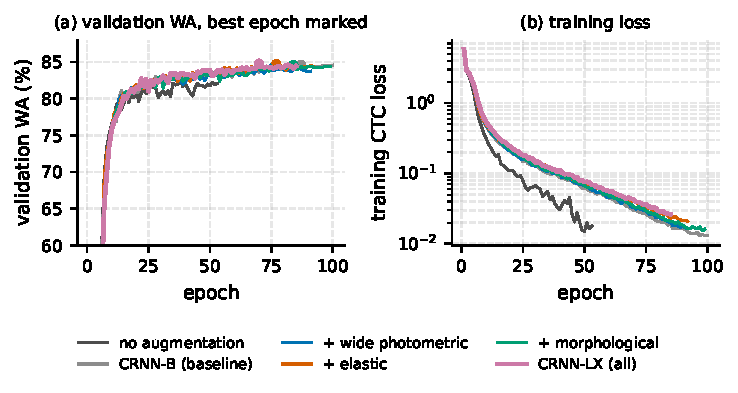
\includegraphics[width=\linewidth]{figures/fig2_training_curves.pdf}
\caption{Training dynamics of the six configurations: (a) validation
word accuracy with the best epoch marked, (b) training CTC loss. The
zero-augmentation anchor reaches the lowest training loss and the
lowest validation accuracy; the five augmented curves coincide.}
\label{fig:curves}
\end{figure}

\subsection{Lexicon Ablation}
\label{sec:res-lex}

Table~\ref{tab:lexicon} holds the optical model fixed (\ours, best
checkpoint) and varies only what happens after greedy decoding. The
effect is an order of magnitude larger than that of the augmentation.
The corrector has two ingredients --- the lexicon a hypothesis is
tested against, and the frequency prior used to rank the candidates
within edit distance --- and the table varies them independently, so
that rows 2 and 4 isolate coverage at fixed rescoring while rows
2$\to$3 and 4$\to$5 isolate the prior at a fixed lexicon.

Coverage decides the sign. Against the training vocabulary alone,
accuracy \emph{falls} from \rawwa\ to 76.42\%: valid English words
absent from the 7\,K training list --- 15\% of the test tokens ---
are forced onto the nearest training word, and most of those
substitutions are wrong. Replacing it with 239\,K types, which cover
94\% of the tokens, turns $-2.41$\,pp into $+0.68$\,pp, a swing of
3.09\,pp at identical rescoring.

The frequency prior supplies most of the magnitude, and its value
grows with the lexicon. On the 7\,K list it is worth $+0.62$\,pp
(76.42 to 77.04\%); on the 239\,K list, $+1.23$\,pp (79.51 to
\ourwa). Fig.~\ref{fig:lexdecomp} shows both effects at once;
Section~\ref{sec:disc-lex} explains why the second grows. Neither
ingredient alone reaches the $+1.91$\,pp of the full corrector.
The pattern holds on the other four augmented optical models of
Table~\ref{tab:main}: the training lexicon costs 2.4--2.7\,pp, the
extended lexicon gains 0.3--0.7\,pp over lexicon-free decoding, the
prior adds a further 1.1--1.3\,pp, and the complete corrector gains
1.5--1.9\,pp. On the zero-augmentation anchor, whose greedy output is
4.4\,pp weaker, the ordering is unchanged but every effect is larger
and the complete corrector gains 3.54\,pp: the more the optical model
errs, the more a lexical prior has to repair.

\begin{table}[t]
\caption{Post-correction ablation with the optical model fixed (\ours\
checkpoint, $N=\nsamples$). Each row applies a different
post-correction to the \emph{same} greedy hypotheses; lexicon size and
n-gram rescoring vary independently.}
\label{tab:lexicon}
\centering
\resizebox{\columnwidth}{!}{%
\begin{tabular}{lrccc}
\toprule
Post-correction & Lexicon size & WA (\%) & CER (\%) & Wilson 95\% CI \\
\midrule
none (\oursnolm, greedy CTC)              & n/a      & 78.83 & \textbf{8.60} & [78.27,\,79.39] \\
training lexicon, edit distance only      & 7\,173   & 76.42 & 11.19 & [75.83,\,76.99] \\
training lexicon $+$ n-gram scoring       & 7\,173   & 77.04 & 10.94 & [76.46,\,77.61] \\
extended lexicon, edit distance only      & 239\,126 & 79.51 & 9.71 & [78.95,\,80.06] \\
\textbf{extended lexicon $+$ n-gram} (\ours) & 239\,126 & \textbf{80.74} & 9.09 & [80.19,\,81.28] \\
\bottomrule
\end{tabular}}
\end{table}

\begin{figure}[t]
\centering
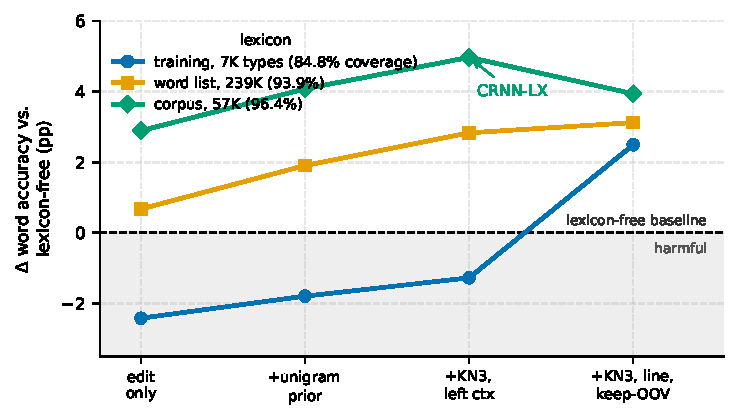
\includegraphics[width=0.82\linewidth]{figures/fig4_lexicon_decomposition.pdf}
\caption{What the post-corrector contributes, measured against lexicon-free
decoding. Coverage decides the sign: with 7\,K types both variants fall
below the baseline, with 239\,K both rise above it. The vertical gap
between the two lines is the contribution of the n-gram prior, and it
doubles as the lexicon grows. Thick lines: the \ours\ optical model;
faint lines: the other five configurations of Table~\ref{tab:main}.}
\label{fig:lexdecomp}
\end{figure}

The character error rate moves the other way: the lexicon-free output
has the lowest CER (\rawcer), and every corrector raises it. A
whole-word corrector can only substitute a complete lexicon entry, so
a wrong replacement turns a near-miss into a different word. The
training lexicon, which replaces many correct-but-unlisted words, pays
this price most heavily (11.19\%); the extended lexicon pays it rarely
(9.09\%) but still raises CER by half a point while improving WA by
almost two. Lexicon-assisted word accuracy and character error rate
therefore measure different things and should be reported together.

\subsection{Comparison with Prior Word-Level Systems}
\label{sec:res-prior}

Table~\ref{tab:priorwork} places \ours\ next to seven published
word-level systems and states, for each, whether a lexicon or language
model was applied at test time. The upper block lists results obtained
on the Aachen writer-disjoint partition. The closest match in protocol
is the sequence-to-sequence recogniser of Sueiras et
al.~\cite{sueiras2018offline}: the sizes of their partition
(47\,952, 20\,306 and 7\,558 words, as compiled
in~\cite{mondal2022yolo}) are those of the \texttt{ok}-filtered Aachen
training, test and validation lists (47\,999, 20\,310 and 7\,559) from
which ours are drawn, and they report lexicon-free word and character
error rates on the full test partition exactly as we do. Under
lexicon-free decoding \oursnolm\ is 2.6\,pp more accurate (\rawwa\
against 76.20\%) at a slightly lower CER (\rawcer\ against 8.80\%);
with the extended lexicon \ours\ is 4.5\,pp ahead. \ours\ remains
below the later attention-based systems: 1.8\,pp below Kang et
al.~\cite{kang2018convolve}, 3.4\,pp below the candidate-fusion model
of Kang et al.~\cite{kang2021candidate} and 3.9\,pp below
AttentionHTR~\cite{kass2022attentionhtr}, which additionally transfers
knowledge from 14.4\,M scene-text images; against our lexicon-free
figure each gap is 1.9\,pp wider. The gap is larger at character level
(5.79--6.88\% against our 8.60--9.09\%), consistent with the
autoregressive decoders of those systems modelling inter-character
dependencies that a CTC output with whole-word post-correction cannot.
The lower block reports three systems measured on other partitions of
IAM; \ours\ is above all three and \oursnolm\ above two, but the
partitions differ in writer overlap and size and we draw no conclusion
from margins of this size.

\begin{table}[t]
\caption{Word-level results on IAM. WA in parentheses is derived as
$1-\mathrm{WER}$ from the cited paper. Lexicon: lexical constraint at
test time (none = unconstrained decoding; LM = language model without
a closed lexicon; n/s = not stated).}
\label{tab:priorwork}
\centering
\resizebox{\columnwidth}{!}{%
\begin{tabular}{llccc}
\toprule
System & Year & Lexicon & WA (\%) & CER (\%) \\
\midrule
\multicolumn{5}{l}{\emph{Aachen writer-disjoint partition ($\approx$20.3\,K test words)}} \\
Sueiras et al.~\cite{sueiras2018offline}      & 2018 & none & (76.20) & 8.80 \\
Kang et al.~\cite{kang2018convolve}           & 2018 & none & (82.55) & 6.88 \\
Kang et al.~\cite{kang2021candidate}          & 2021 & LM   & (84.09) & \textbf{5.79} \\
Kass and Vats~\cite{kass2022attentionhtr}     & 2022 & none & (\textbf{84.60}) & 6.50 \\
\oursnolm\ (ours)                             & 2026 & none & 78.83 & 8.60 \\
\textbf{\ours} (ours)                         & 2026 & 239\,K general & 80.74 & 9.09 \\
\midrule
\multicolumn{5}{l}{\emph{Other partitions of IAM}} \\
Mondal et al.~\cite{mondal2022yolo}$^{a}$                                    & 2022 & none & (70.79) & 9.53 \\
CNN--RNN of~\cite{dutta2018improving}, re-trained in~\cite{rajesh2022hwrcnet}$^{b}$ & 2022 & n/s & (77.14) & 11.08 \\
Rajesh et al.~\cite{rajesh2022hwrcnet}$^{b}$                                 & 2022 & n/s & 80.08 & 9.89 \\
\bottomrule
\multicolumn{5}{l}{\footnotesize $^{a}$30\,K randomly selected test words; 1\,200 training images.} \\
\multicolumn{5}{l}{\footnotesize $^{b}$Random 95:5 split, writer-dependent, $\approx$5.8\,K test words.} \\
\end{tabular}}
\end{table}

\subsection{Error Analysis}
\label{sec:res-err}

\ours\ misrecognises 3\,912 of the \nsamples\ test words. Only 274 of
them (7.0\%) differ from the reference in letter case alone; the
remaining errors are genuine. At character level the aligned errors
consist of 5\,244 substitutions, 1\,804 deletions and 394 insertions,
so the model drops characters far more often than it hallucinates
them. Fig.~\ref{fig:confusion} shows the ten most frequent
substitutions: they are symmetric confusions between visually similar
lower-case glyphs --- \texttt{o}$\leftrightarrow$\texttt{a} (242
cases), \texttt{s}$\leftrightarrow$\texttt{r} (150),
\texttt{n}$\leftrightarrow$\texttt{r} (98),
\texttt{n}$\leftrightarrow$\texttt{m} (98),
\texttt{t}$\leftrightarrow$\texttt{l} (97),
\texttt{e}$\leftrightarrow$\texttt{a} (86).
Case substitutions account for 7.7\% of all substitutions. These are
errors of shape, not of vocabulary: a whole-word lexicon repairs them
only when the mis-shaped word falls outside the lexicon and its correct
form lies within two edits --- the population that the extended lexicon
recovers in Table~\ref{tab:lexicon}.

\begin{figure}[t]
\centering
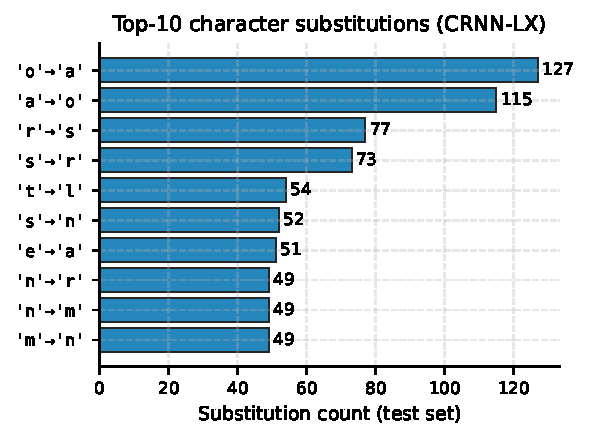
\includegraphics[width=0.85\linewidth]{figures/fig3_confusion_topk.pdf}
\caption{Ten most frequent character substitutions of \ours\ on the
test set (true\,$\rightarrow$\,predicted).}
\label{fig:confusion}
\end{figure}

% ---- 6. Discussion ------------------------------------------------------
\section{Discussion}
\label{sec:discussion}

\subsection{Why the Augmentation Does Not Help Here}

The anchor answers the objection that would otherwise be hardest to
rebut: that a single-seed experiment is too noisy to see anything. The
same test, data and seed detect the removal of the conventional
pipeline at $p=2\times10^{-27}$. The apparatus is not blind to
augmentation; it is blind to \emph{these} transforms on \emph{this}
training set. Three observations locate the saturation.

First, the anchor overfits and the augmented runs do not: training
loss 0.018 against 0.09--0.11, early stopping 30 epochs sooner
(Fig.~\ref{fig:curves}). The first increment of augmentation buys
regularisation that the network genuinely needs. Second, among the
augmented configurations the validation curves coincide and the extra
transforms neither slow convergence nor raise the plateau, while the
fully augmented model reaches a slightly higher training loss --- so
they do regularise further, but the baseline is no longer overfitting
in a way that costs accuracy on unseen writers. Third, the per-word
disagreements between those configurations are large yet balanced.
Together these indicate that with 48\,K training words from 283
writers, the writer-to-writer variation already present in the data
exceeds what elastic and morphological perturbation of 64-pixel-high
crops can add on top of affine and photometric jitter. Reports of
sizeable gains from such augmentation, including our own preliminary
experiments, came from smaller training sets or from comparisons in
which augmentation was not the only difference. The result does not
imply that augmentation is useless for HTR in general --- Wigington et
al.~\cite{wigington2017data} report gains on lines with a different
transform family, and our own anchor shows the first increment is
worth 2.5\,pp --- but it does show that further transforms must be
measured under controlled conditions before being claimed.

\subsection{Coverage and the Frequency Prior}
\label{sec:disc-lex}

The ablation separates two effects that are usually conflated under
``adding a language model'', and they turn out to do different jobs.
Membership testing against a list that covers 85\% of the test tokens
is harmful, because the corrector cannot distinguish a misrecognised
word from a correctly recognised word it has never seen and treats
both as errors; raising coverage to 94\% is what turns the loss into
a gain. That gain is small on its own, however. What converts it into
the full $+1.9$\,pp is the prior that ranks the candidates, and it is
worth twice as much on the large lexicon as on the small one.

At the word level the prior cannot be doing linguistic work: an
isolated crop offers no context, so the trigram backs off to unigram
frequency. What it does instead is break ties. The tighter the
lexicon, the fewer entries lie within two edits of a hypothesis and
the less the ranking matters; at 239\,K types a mis-shaped word
typically has several equidistant neighbours, and picking the frequent
one is right more often than picking an arbitrary one. Edit distance identifies the candidate set and
frequency chooses inside it.

A practical consequence is that word-level HTR results obtained with a
closed lexicon should state both the lexicon's coverage of the test
vocabulary and the rule used to rank candidates, without which the
reported accuracy is not interpretable. The remaining 6\% of uncovered tokens --- proper nouns,
rare inflections, punctuation-bearing strings --- bound what any
whole-word corrector can achieve.

\subsection{Comparison with Sueiras et al.}
\label{sec:disc-sueiras}

The recogniser of Sueiras et al.~\cite{sueiras2018offline} is the
published result whose protocol matches ours most closely, and the
only one for which we could verify the match from the reported
partition sizes (Section~\ref{sec:res-prior}): isolated IAM words, the
Aachen writer-disjoint partition drawn from the same
\texttt{ok}-filtered word lists, and lexicon-free error rates on the
full test partition. Architecturally the two differ in every stage: they extract features from a sliding window
of image patches with a LeNet-5-style convolutional network and
transcribe them with a recurrent encoder--decoder using attention,
whereas \oursnolm\ is a single convolutional-recurrent network trained
with CTC. Under lexicon-free decoding \oursnolm\ reaches \rawwa\
against their 76.20\% (23.8\% word error rate), a margin of 2.6\,pp
that is almost five times the half-width of our confidence interval,
at a slightly lower character error rate (\rawcer\ against 8.80\%).
Post-correction with the extended lexicon widens the word-level margin
to 4.5\,pp. Sueiras et al. also report lexicon-constrained variants of
their recogniser; those depend on the lexicon employed and are not
compared here. We read the comparison as evidence that a plain CRNN
trained from scratch on the 48\,K Aachen training words is competitive
with an early attention model under the same protocol --- not as
evidence about augmentation, which Table~\ref{tab:main} shows
contributes nothing measurable to the margin.

HWRCNet~\cite{rajesh2022hwrcnet}, the closest system in construction
(a CNN, a bidirectional LSTM and a CTC layer), reports 80.08\% strict
word accuracy, 0.66\,pp below \ours\ and 1.25\,pp above \oursnolm. It
is measured on a random 95:5 partition whose test set is
writer-dependent and about 3.5 times smaller than ours, so neither
difference is interpretable.

\subsection{Threats to Validity}

Each configuration was trained once. The augmentation differences of
0.0--0.4\,pp are below what a single seed can resolve, which is why we
report them as non-significant rather than as small gains; establishing
an effect of that size would require several seeds per configuration.
The $2.49$\,pp effect of the conventional pipeline is an order of
magnitude larger than that resolution limit, so the positive control
does not depend on the seed in the way the null result does.
The lexicon and rescoring effects ($-2.4$ to $-2.7$\,pp for the
training vocabulary, $+1.1$ to $+1.3$\,pp for the frequency prior) are
reproduced in sign and ordering on all six independently trained
models and are well outside the interval, although their magnitude
grows as the optical model weakens. They are, however, measured with one corrector
and one word list; another edit-distance bound or general vocabulary
would change their size, if not their ordering.
Validation accuracy exceeds test accuracy by about four points for
every configuration; the validation writers are used for checkpoint
selection and are only 55 in number, so this gap is expected and does
not indicate a fault. The external systems in Table~\ref{tab:priorwork}
were trained and evaluated by their authors with their own
preprocessing and, in the lower block, on a different partition; we
therefore treat only our own six configurations as a controlled
comparison. Finally, the extended lexicon is a general English word
list and contains no IAM test transcriptions, but it is a closed
lexicon nonetheless, and \ours\ should be read as a lexicon-assisted
result.

% ---- 7. Conclusion ------------------------------------------------------
\section{Conclusion}
\label{sec:conclusion}

\ours\ recognises isolated handwritten words with \ourwa\ accuracy
(\ourcer\ character error rate) on the complete Aachen writer-disjoint
test set of IAM, with a plain CRNN trained from scratch and no external
image data. Under the same partition and lexicon-free decoding it is
2.6\,pp more accurate than the sequence-to-sequence recogniser of
Sueiras et al.~\cite{sueiras2018offline} and 2--4\,pp less accurate
than later attention-based systems. Under controlled conditions, elastic deformation,
morphological perturbation and a widened photometric range do not
change this figure measurably, while removing the conventional
augmentation pipeline beneath them costs $2.49$\,pp --- the benefit of
augmentation saturates well before the transforms we proposed; a
widely used elastic parameterisation, moreover, does not deform the
image at all. The post-correction stage, by
contrast, moves accuracy by two points in either direction: its
lexicon's coverage of the test vocabulary decides whether the
correction helps or hurts, and the frequency prior that ranks the
candidates supplies most of the gain once coverage is sufficient.
Both improve word accuracy at the expense of character error rate.

For word-level HTR the practical conclusions are that an ablation
reporting no effect should include a configuration in which the effect
is known to exist; that lexicon coverage and candidate ranking should
be reported separately alongside lexicon-assisted accuracy; and that
word accuracy and character error rate should be given together
whenever a whole-word corrector is used. Future work
will test whether the augmentation becomes useful in the low-data
regime, replace the whole-word corrector with a character-level
open-vocabulary model to address the uncovered 6\% of tokens, and
evaluate the pipeline on text lines, where n-gram context is
available.

% ---- Acknowledgements ---------------------------------------------------
\section*{Acknowledgements}
We thank the maintainers of the IAM Handwriting Database and of the
Aachen split.

% ---- References ---------------------------------------------------------
\bibliographystyle{IEEEtran}
\bibliography{references}

\end{document}
